\documentclass[letter,11pt]{article}

\usepackage[spanish,es-nodecimaldot]{babel}
\usepackage[utf8]{inputenc}

\usepackage{lmodern}
\usepackage[T1]{fontenc}
\usepackage{textcomp}

\usepackage{framed}
\usepackage[svgnames]{xcolor}
\colorlet{shadecolor}{Gainsboro!50}

\usepackage[labelfont=bf]{caption}
\usepackage{graphicx}
\usepackage{pstricks}

\usepackage{anysize}
\marginsize{3cm}{2cm}{2cm}{3cm}

\usepackage{siunitx}
\usepackage{amsmath}
\usepackage{array}
\usepackage{xcolor,colortbl}

\usepackage{fancyhdr}
\usepackage{lastpage}
\pagestyle{fancy}
\fancyhf{}
\fancyhead[LE,RO]{Laboratorio de Física Básica III}
\fancyfoot[CO,CE]{\thepage\ de \pageref{LastPage}}

\special{papersize=215.9mm,279.4mm}

\usepackage[
    pdfauthor={
        Bastos Lizondo Rosemary;
        Blanco Alconz John Brandon;
        Caballero Burgoa Carlos Eduardo;
        Villena Gutiérrez Ismael Cristian
    },%
    pdftitle={Laboratorio de Física Básica III},%
    pdfsubject={Circuitos eléctricos en D.C. y leyes de Kirchhoff},%
    colorlinks,%
    citecolor=black,%
    filecolor=black,%
    linkcolor=black,%
    urlcolor=black,
    breaklinks]{hyperref}
\usepackage{breakurl}

\newcommand{\blankpage}{
\newpage
\thispagestyle{empty}
\mbox{}
\newpage
}

\renewcommand{\arraystretch}{1.2}

\begin{document}

\begin{titlepage}
\begin{center}
{\Large UNIVERSIDAD MAYOR DE SAN SIMÓN}\\
\vspace*{0.15cm}
{\large FACULTAD DE CIENCIAS Y TECNOLOGÍA}\\
\vspace*{0.10cm}
DEPARTAMENTO DE FÍSICA\\
\vspace*{3.0cm}
{\Large \textbf{LABORATORIO DE FÍSICA BÁSICA III}}\\
\vspace*{0.3cm}
{\Large \textbf{INFORME No. 6}}\\
\vspace*{3.5cm}
{\Large \textbf{CIRCUITOS ELÉCTRICOS EN D.C. \\ Y LEYES DE \emph{KIRCHHOFF}}}\\
\end{center}

\vspace*{5.8cm}
\leftskip=7.95cm
\noindent
\textbf{Integrantes:}\\
Bastos Lizondo Rosemary.\\
Blanco Alconz John Brandon.\\
Caballero Burgoa Carlos Eduardo.\\
Villena Gutiérrez Ismael Cristian.\\
\newline
\textbf{Docente:}\\
Ing. Flores Flores, Freddy.\\
\newline
\textbf{Grupo:} G3.\\
\textbf{Fecha de entrega:} 13 de Mayo del 2021.\\

\end{titlepage}

\section{Preguntas previas}
\begin{enumerate}
\item \textbf{Enunciar las leyes de \emph{Kirchhoff}.} \\
Consisten en los dos siguientes enunciados:

\begin{description}
\item [Regla de \emph{Kirchhoff} de los nodos:]
La suma algebraica de las corrientes en cualquier nodo es igual a cero.

\begin{equation*}
    \sum I = 0
\end{equation*}

\item [Regla de \emph{Kirchhoff} de las mallas:]
La suma algebraica de las diferencias de potencial en cualquier malla, incluso
las asociadas con las FEM y las de elementos con resistencia, debe ser igual a
cero.

\begin{equation*}
    \sum V = 0
\end{equation*}

\end{description}

\item \textbf{Aplicando las leyes de \emph{Kirchhoff}, resolver el circuito DC
de la Figura \ref{figura1}} \\
Usando las leyes de \emph{Kirchhoff}, y considerando las direcciones de la
corriente descritos en la \textbf{Figura \ref{figura4}}, se plantean las
siguientes condiciones:

\underline{De la ley de nodos}:

\begin{equation*}
    I_1 = I_2 + I_3
\end{equation*}

\underline{De la ley de mallas}:

\begin{equation*}
    V - R_i I_1 - R_1 I_1 - R_3 I_3 - R_4 I_1 = 0
\end{equation*}
\begin{equation*}
    -R_2 I_2 + R_3 I_3 = 0
\end{equation*}

Se obtiene un sistema de ecuaciones lineales de 3 incógnitas:

\begin{equation*}
    \begin{cases}
        I_1 - I_2 - I_3 = 0 \\
        (R_i + R_1 + R_4) I_1 + R_3 I_3 = V \\
        R_2 I_2 - R_3 I_3 = 0
    \end{cases}
\end{equation*}

\item \textbf{¿Cómo se puede calcular la potencia disipada en un resistor?} \\
Una resistencia, cuando se utiliza en un circuito, crea una caída de voltaje
limitando la cantidad de potencia que pasa a través de él. La potencia extra se
disipa en forma de energía calórica. La cantidad de potencia disipada puede ser
calculada utilizando una fórmula derivada de la ley de \emph{Ohm}.

\begin{equation*}
    P = V\,I = R\,I^2 = \frac{V^2}{R}
\end{equation*}

\item \textbf{¿Qué cuidados se deben tener con el voltímetro y amperímetro al
medir el voltaje y la corriente eléctrica en un circuito DC?} \\
Se debe tener en cuenta que el voltímetro se conecta en paralelo al circuito a
medir, mientras que el amperímetro debe ser conectado en serie.

\end{enumerate}

\section{Objetivos}

\begin{figure}[!h]
\centering
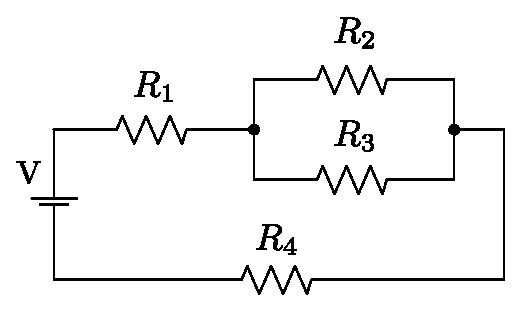
\includegraphics[scale=0.85]{resources/figura1.eps}
\caption{Circuito eléctrico en DC.}
\label{figura1}
\end{figure}

\begin{itemize}
\item Resolver el circuito de la \textbf{Figura \ref{figura1}} a través de
mediciones de voltaje y corriente eléctrica.
\item Aplicar la ley de \emph{Ohm} y las leyes de \emph{Kirchhoff} para resolver
el circuito de la \textbf{Figura \ref{figura1}}.
\end{itemize}

\section{Fundamento teórico}

Para resolver circuitos donde existan varios nodos o más de una malla, es
necesario aplicar las leyes de \emph{Kirchhoff}:

\subsection{Primera ley de \emph{Kirchhoff}, ley de corrientes}

La primera ley de \emph{Kirchhoff} está fundamentada con la conservación de la
carga eléctrica, y establece:

\begin{quote}
``Para todo nodo, la suma de las corrientes que entran, es igual a la suma de
las corrientes que salen, es decir, la suma algebraica de las corrientes que
pasa por un nodo es igual a cero''.
\end{quote}

\begin{equation}
    \sum_{i=1}^{n} I_i = 0
\label{kirchhoff1}
\end{equation}

\subsection{Segunda ley de \emph{Kirchhoff}, ley de mallas}

La segunda ley de \emph{Kirchhoff} está fundamentada con la conservación de la
energía, y establece:

\begin{quote}
``Para una malla, la suma algebraica de las diferencias de potencial eléctrico
es igual a cero''.
\end{quote}

\begin{equation}
    \sum_{i=1}^{n} V_i = 0
\label{kirchhoff2}
\end{equation}

\subsection{Potencia eléctrica}

La potencia eléctrica generada por un dispositivo de dos terminales es:

\begin{equation}
    P = V\, I
\label{potencia1}
\end{equation}

Con la ley de \emph{Ohm}, se tiene:

\begin{equation}
    P = R\,I^2 = \frac{V^2}{R}
\label{potencia2}
\end{equation}

\section{Materiales}

\begin{itemize}
\item Simulador «PhET Interactive Simulations» Kit de Construcción de Circuitos:
CD - Laboratorio Virtual.
\end{itemize}

\section{Procedimiento experimental}

A continuación se describe el procedimiento experimental que se llevará a cabo:

\begin{figure}[!h]
\centering
\includegraphics[scale=0.45]{resources/figura2.eps}
\caption{Simulador para el montaje de circuitos.}
\label{figura2}
\end{figure}

\begin{enumerate}
\item Ir al simulador ubicado en la dirección web:
(https://phet.colorado.edu/sims/html/circuit-construction-kit-dc-virtual-lab/latest/circuit-construction-kit-dc-virtual-lab\_es.html),
tal como se muestra en la \textbf{Figura \ref{figura2}}.
\item Establecer los valores de las resistencias a utilizar,
\item Establecer un valor adecuado de la fuente de alimentación DC y su
    resistencia interna para el circuito de la \textbf{Figura \ref{figura1}}.
\item Con el voltímetro, medir el voltaje en cada resistencia.
\item Con el amperímetro medir las corrientes que circulan por cada resistencia.
\item Calcular las potencias disipadas en cada resistencia.
\end{enumerate}

\section{Resultados}

\begin{figure}[!h]
\centering
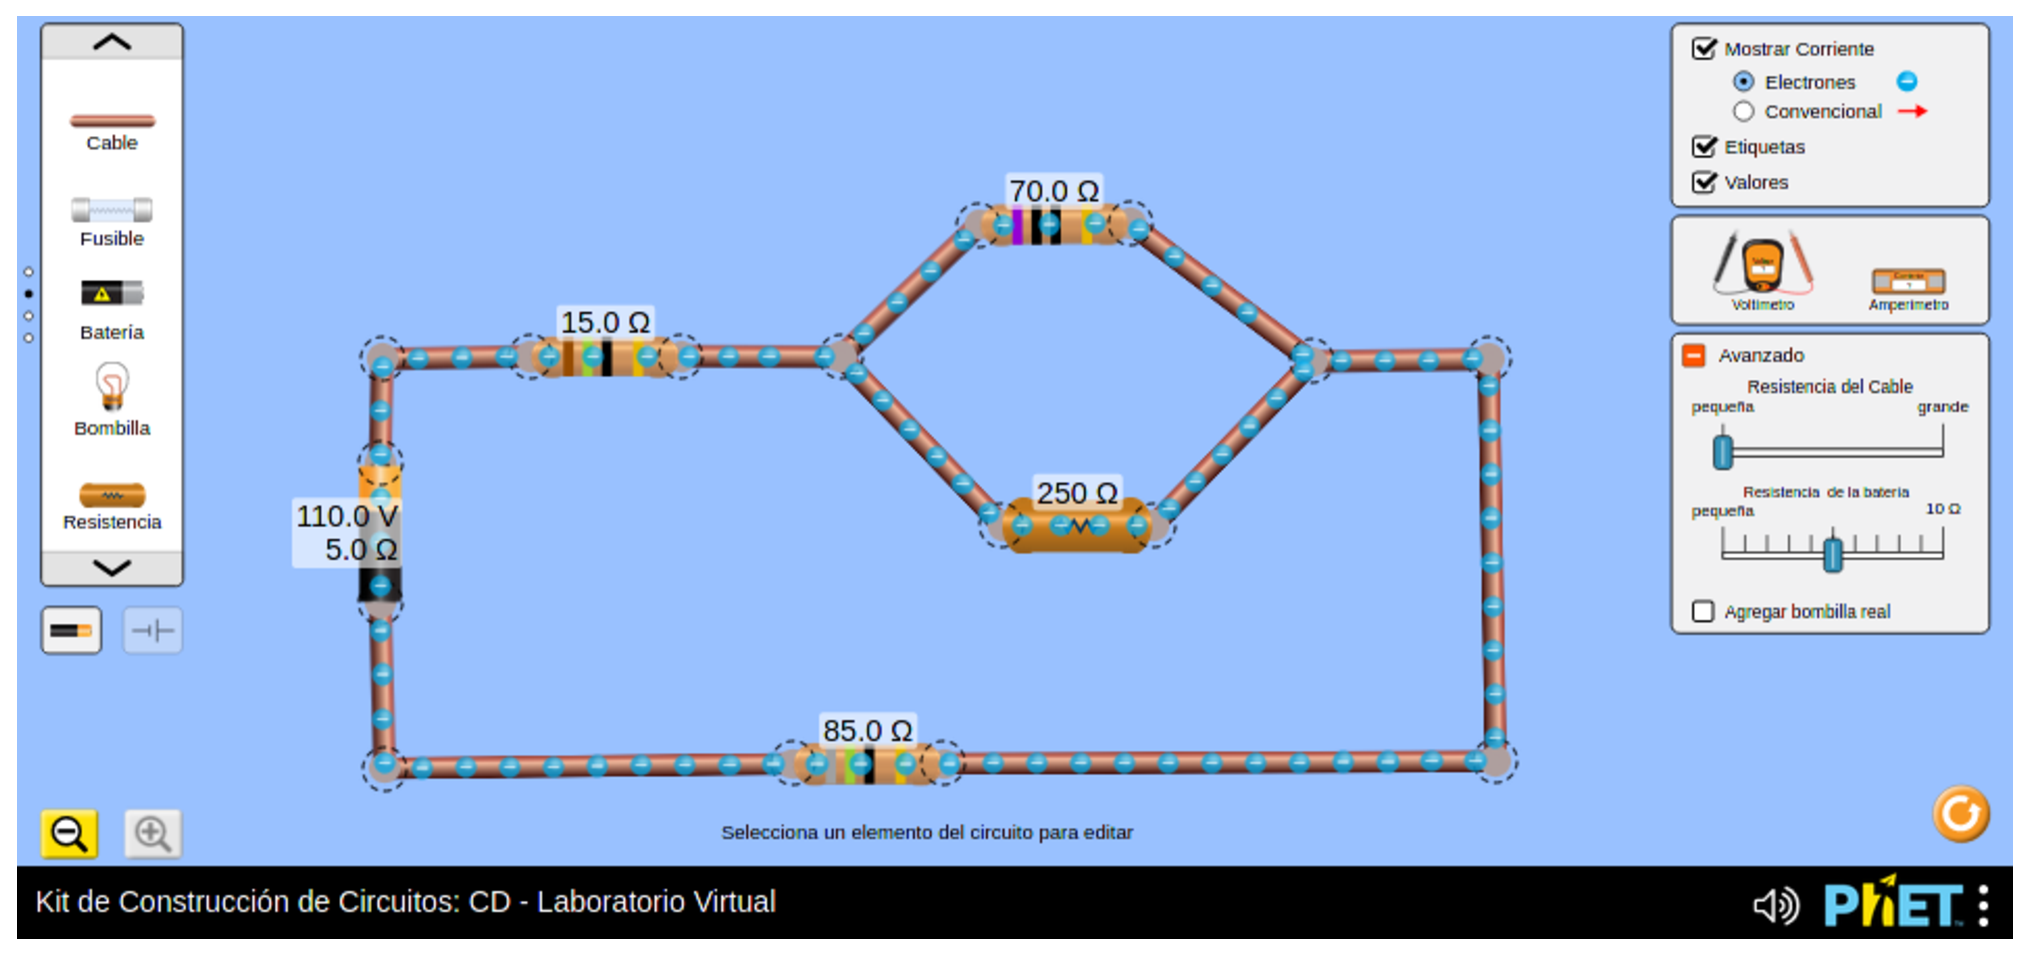
\includegraphics[scale=0.45]{resources/figura3.eps}
\caption{Circuito usado para el experimento.}
\label{figura3}
\end{figure}

En la \textbf{Figura \ref{figura3}} se presenta el armado del circuito realizado
en el simulador.

Voltaje de la batería:

\begin{equation*}
    V = 110 [V]
\end{equation*}

Resistencia interna de la batería:

\begin{equation*}
    R_i = 5.0 [\Omega]
\end{equation*}

En el \textbf{Cuadro \ref{cuadro1}} se presentan los valores de las resistencias
elegidas, asimismo las mediciones de corrientes, voltaje, y el calculo de las
potencias eléctricas para cada resistencia.

\begin{table}[!h]
\begin{center}
\begin{tabular}{|c|>{\centering}m{2.75cm}<{\centering}|
                  |>{\centering}m{2.75cm}<{\centering}
                  |>{\centering}m{2.75cm}<{\centering}|
                  |>{\centering}m{2.75cm}<{\centering}|}
\hline
& Resistencia $[\Omega]$ & Corriente $[A]$ & Voltaje $[V]$ & Potencia $[W]$
    \tabularnewline \hline \hline
1 &  15.0 & 0.66 & 10.33 &  6.82 \tabularnewline \hline
2 &  70.0 & 0.51 & 37.67 & 19.21 \tabularnewline \hline
3 & 250.0 & 0.15 & 37.67 &  5.65 \tabularnewline \hline
4 &  85.0 & 0.65 & 58.56 & 38.06 \tabularnewline \hline
\end{tabular}
\caption{Valores de la corriente eléctrica, voltaje y potencia eléctrica.}
\label{cuadro1}
\end{center}
\end{table}

Para el cálculo de los valores en el circuito usando las leyes de
\emph{Kirchhoff}, se consideran los sentidos de la corriente mostrados en la
\textbf{Figura \ref{figura4}}.
 
\begin{figure}[!h]
\centering
\includegraphics[scale=0.85]{resources/figura4.eps}
\caption{Elección del sentido de las corrientes para el circuito.}
\label{figura4}
\end{figure}

Se obtiene el siguiente sistema de ecuaciones:

\begin{equation*}
    \begin{cases}
        I_1 - I_2 - I_3 = 0 \\
        105 I_1 + 250 I_3 = 110 \\
        70 I_2 - 250 I_3 = 0
    \end{cases}
\end{equation*}

Resolviendo el sistema de ecuaciones, se obtiene:

\begin{equation*}
    I_1 = 0.6888 [A]
\end{equation*}
\begin{equation*}
    I_2 = 0.5382 [A]
\end{equation*}
\begin{equation*}
    I_3 = 0.1507 [A]
\end{equation*}

Aplicando las leyes de \emph{Kirchhoff} y conocidos los valores de las
resistencias y el voltaje de la fuente de tensión, se obtienen los datos
presentados en el \textbf{Cuadro \ref{cuadro2}}.

\begin{table}[!h]
\begin{center}
\begin{tabular}{|c|>{\centering}m{2.75cm}<{\centering}|
                  |>{\centering}m{2.75cm}<{\centering}
                  |>{\centering}m{2.75cm}<{\centering}|
                  |>{\centering}m{2.75cm}<{\centering}|}
\hline
& Resistencia $[\Omega]$ & Corriente $[A]$ & Voltaje $[V]$ & Potencia $[W]$
    \tabularnewline \hline \hline
1 &  15.0 & 0.69 & 10.33 &  7.12 \tabularnewline \hline
2 &  70.0 & 0.54 & 37.67 & 20.27 \tabularnewline \hline
3 & 250.0 & 0.15 & 37.67 &  5.68 \tabularnewline \hline
4 &  85.0 & 0.69 & 58.55 & 40.33 \tabularnewline \hline
\end{tabular}
\caption{Valores de la corriente eléctrica, voltaje y potencia eléctrica.}
\label{cuadro2}
\end{center}
\end{table}

\section{Cuestionario}

\begin{enumerate}
\item \textbf{Demostrar que la corriente $I_{R_1} = I_{R_4}$.} \\
En el circuito eléctrico solo existen dos nodos ($a$ y $b$).

Entonces según la ley de nodos, la corriente que sale de $b$ es equivalente a la
que entra en $a$.

Por tanto:

\begin{equation*}
    I_1 = I_{R_1} = I_{R_4}
\end{equation*}

\item \textbf{Demostrar que $V_{R_2} = V_{R_3}$}. \\
La resistencia $R_2$ y la resistencia $R_3$ son los únicos componentes que
integran la malla $2$.

Entonces según la ley de mallas, la suma de ambos voltajes debe ser igual a $0$.

Por tanto:

\begin{equation*}
    \sum V_i = V_{R_2} - V_{R_3} = 0
\end{equation*}
\begin{equation*}
    V_{R_2} = V_{R_3}
\end{equation*}

\item \textbf{Demostrar que $P_T = P_{R_1} + P_{R_2} + P_{R_3} + P_{R_4}$}. \\

Simplificando el circuito a una resistencia equivalente:

\begin{equation*}
    \frac{1}{R_{23}} = \frac{1}{R_2} + \frac{1}{R_3}
\end{equation*}
\begin{equation*}
    R_{23} = 54.687 [\Omega]
\end{equation*}
\begin{equation*}
    R_T = R_i + R_1 + R_{23} + R_4 = 159.69 [\Omega]
\end{equation*}

Por tanto:

\begin{equation*}
    P_T = \frac{V^2}{R_T} = 75.773 [W]
\end{equation*}

La suma de las potencias individuales es:

\begin{equation*}
    \sum P_i = P_1 + P_2 + P_3 + P_4 + R_i I^2_1
             = 73.400 + (5)(0.69)^2 = 75.773 [W]
\end{equation*}

\item \textbf{Para la parte experimental si el voltaje de la fuente de tensión
    incrementa, ¿Qué cuidados se deben tener con las resistencias
    eléctricas?} \\

De la ley de \emph{Ohm} se sabe:

\begin{equation*}
    V = I\, R
\end{equation*}

Por tanto:

\begin{equation*}
    I = \frac{1}{R} V
\end{equation*}

La corriente eléctrica se incrementará proporcionalmente al incremento del
voltaje.

Entonces se debe tener cuidado de no exceder el valor de la corriente de
cortocircuito de las resistencias que componen el circuito.

\end{enumerate}
 
\end{document}

